\section{Evaluation}
\label{sec:evaluation}

This section presents our experimental evaluation of \GreenFaaS{}
against four carbon-aware baselines. \S\ref{sec:evaluation:methodology}
describes the trace data and reconstruction methodology.
\S\ref{sec:evaluation:headline} reports headline results.
\S\ref{sec:evaluation:topology}--\S\ref{sec:evaluation:intensity}
sweep five sensitivity axes (topology, SLA mix, forecast accuracy,
carbon variability, workload intensity).
\S\ref{sec:evaluation:summary} synthesizes the cross-axis findings.

\subsection{Methodology}
\label{sec:evaluation:methodology}

\paragraph{Workload traces.} Our evaluation uses two kinds of
workload. The controlled sensitivity sweeps
(\S\ref{sec:evaluation:sla}--\S\ref{sec:evaluation:intensity}) are
driven by a schema-faithful \emph{synthetic} workload, because their
purpose is to vary individual parameters (SLA mix, forecast accuracy,
carbon variability, arrival rate) cleanly across wide ranges. The
fully-real validation (\S\ref{sec:evaluation:realboth}) is driven by
the real \emph{Azure Functions Invocation Trace 2021}
\citep{zhang2021faster,azuretrace}, a per-invocation trace with schema
\code{(app, func, end\_timestamp, duration)}; the 2021 loader converts
each row to an \code{Invocation} by computing
\code{arrival\_time = end\_timestamp - duration} and mapping
\code{(app, func)} pairs to stable function IDs. Our loaders also
accept the \emph{Azure Functions 2019} dataset
\citep{shahrad2020serverless}, which is \emph{aggregated} (per-minute
invocation counts plus per-function duration percentiles); the 2019
loader reconstructs a per-invocation stream by drawing arrival times
uniformly within each minute bin and sampling per-invocation durations
from the empirical percentile distribution via linear inverse-CDF
interpolation. Both loaders accept the exact published schemas, so the
same evaluation code runs end-to-end on either real or synthetic
input.

\paragraph{Synthetic workload calibration.} The synthetic workload
used in the sensitivity sweeps is calibrated to the
\citet{shahrad2020serverless} and \citet{zhang2021faster}
characterizations: non-homogeneous Poisson arrivals with diurnal
shape, Zipf popularity with $s = 1.2$, heavy-tailed durations, and
the SLA mix described below. We use synthetic input for the sweeps
because controlled parameter variation across multiple axes requires
generating workloads the real trace does not contain (e.g. a $25\%$
shiftable fraction, or a forecast-error level of $0.3$); the
fully-real experiment of \S\ref{sec:evaluation:realboth} confirms that
the headline ordering established on synthetic data reproduces on the
real Azure 2021 trace paired with time-aligned real carbon.

\paragraph{Latency-class assignment.} Neither Azure dataset
explicitly labels SLA tiers. For the 2019 trace the loader maps the
explicit \code{Trigger} field: HTTP $\to$ \Interactive; queue,
event-grid, orchestration $\to$ \Deferrable; timer, storage $\to$
\Background. For the 2021 trace (no trigger field) the loader
classifies by observed mean duration: $<1$\,s $\to$ \Interactive{}
(1\,s SLA); 1--30\,s $\to$ \Deferrable{} (60\,s SLA); $>30$\,s $\to$
\Background{} (1\,hour SLA). The synthetic workload uses the same
class distribution as the 2019 trigger-field histogram.

\paragraph{Carbon traces.} We use the publicly-released hourly
carbon-intensity traces from \citet{wiesner2021lets,lwa} (DE, GB, FR,
US-CAISO, 2020), computed from ENTSO-E and CAISO generation-mix data
using IPCC factors. For experiments requiring a coal-belt region
(\S\ref{sec:evaluation:realtopology}) we extend with a calibrated
PL trace whose annual mean (791\,g CO$_2$eq/kWh) matches the value
LWA documents for Poland in 2020 and whose coal-base-load diurnal
shape uses the same generation factors as the LWA computation
pipeline; we label it ``PL (synth., LWA methodology)'' wherever it
appears. The simulator resamples all carbon traces to a uniform
5-minute resolution via linear interpolation.

\paragraph{Baselines.} \textbf{FIFO} (carbon-unaware lower bound).
\textbf{Wait-Awhile} \citep{wiesner2021lets}: temporal deferral with
threshold $C^* = 200$\,g\,CO$_2$eq/kWh. Two variants are reported:
\emph{Wait-Awhile-Batch} (max\_defer = 1800\,s, Wiesner et al.'s
batch-job default) and \emph{Wait-Awhile-FaaS} (max\_defer = 60\,s,
matching \GreenFaaS's \Deferrable{} horizon). The two variants
together address an obvious reviewer concern (\S\ref{sec:evaluation:fair-waitawhile}).
\textbf{Spatial}: route to the lowest-current-carbon region within a
class-dependent RTT budget. \textbf{GreenFaaS-v1}: the
\GreenFaaS{} scheduler \emph{without} the
\S\ref{sec:tradeoff:idle} idle-energy correction, included as an
ablation.

\subsection{Headline Results}
\label{sec:evaluation:headline}

We report headline results on a canonical synthetic experiment and
validate them on real carbon data in \S\ref{sec:evaluation:realcarbon}.
The canonical workload is 24h long with 173k invocations across 5
regions including France as a low-carbon refuge and Poland at the
high-carbon extreme.

\begin{table}[t]
\centering\small
\caption{Synthetic 24h workload, 5 regions, 173k invocations,
\textbf{mean $\pm$ std across 5 seeds} (42--46). Wait-Awhile-Batch
uses the original 1800\,s defer horizon; see
\S\ref{sec:evaluation:fair-waitawhile} for the fair-parameterization
variant.}
\label{tab:headline}
\begin{tabular}{lrr}
\toprule
Scheduler & Carbon (g) & vs FIFO \\
\midrule
FIFO              & 51.57 $\pm$ 0.37 & 0.0\% \\
Wait-Awhile-Batch & 209.66 $\pm$ 2.51 & $-$306.5\% $\pm$ 4.3\% \\
Spatial           & 13.97 $\pm$ 0.07 & \textbf{+72.91\% $\pm$ 0.26\%} \\
GreenFaaS-v1      & 14.73 $\pm$ 0.13 & +71.43\% $\pm$ 0.40\% \\
\GreenFaaS        & 14.52 $\pm$ 0.07 & +71.84\% $\pm$ 0.32\% \\
\bottomrule
\end{tabular}
\end{table}

Three observations frame the rest of \S\ref{sec:evaluation}.
\emph{First}, the batch-oriented Wait-Awhile scheduler with its
default 1800\,s deferral horizon \emph{more than triples} operational
carbon ($-306.5\% \pm 4.3\%$ on synthetic, $-176.2\% \pm 2.5\%$ on
real LWA across 5 seeds), an
empirical confirmation that batch carbon-aware techniques do not
transfer to FaaS. \S\ref{sec:evaluation:fair-waitawhile} shows that
shorter, FaaS-appropriate deferral horizons (60\,s, 30\,s) do not
rescue Wait-Awhile --- they cause it to degenerate to a FIFO no-op,
because its absolute-threshold criterion is rarely met inside such
windows. We attribute the long-horizon failure mode in
\S\ref{sec:evaluation:variability} to the synchronised-defer pile-up
effect noted in \S\ref{sec:tradeoff:idle}. \emph{Second},
\GreenFaaS{} reaches $71.84\% \pm 0.32\%$ reduction relative to FIFO,
within 1.1 percentage points of pure spatial routing
($72.91\% \pm 0.26\%$); the GreenFaaS--Spatial gap is small but
statistically detectable (see the significance paragraph below),
with Spatial consistently edging \GreenFaaS{}. The two schedulers
are indistinguishable on SLA violation rate, p95 latency, and
cold-start rate. \emph{Third}, the ablation between GreenFaaS-v1 and
\GreenFaaS{} shows a meaningful but modest gap on this canonical
workload ($71.43\% \pm 0.40\%$ vs $71.84\% \pm 0.32\%$). The
interesting separation appears not on canonical
workloads but in the sensitivity sweeps of
\S\ref{sec:evaluation:sla} and \S\ref{sec:evaluation:variability},
and in the coal-belt topology
(\S\ref{sec:evaluation:realtopology}) where the ablation's variance
blows up by an order of magnitude (std jumps from 0.4\% to 9.8\%) ---
v1 produces unpredictably bad outcomes when the spatial axis offers
limited refuge.

The real-carbon validation in \S\ref{sec:evaluation:realcarbon}
reproduces the same ordering on real LWA 2020 ENTSO-E / CAISO data,
with magnitudes shifted modestly (GreenFaaS $64.63\% \pm 0.24\%$
reduction vs $\sim 72\%$ on synthetic) because real 2020 European
carbon was cleaner overall than our synthetic calibration assumed.

\paragraph{Statistical significance of the key gaps.}
We report paired statistical tests (paired $t$-test and Wilcoxon
signed-rank) for the load-bearing scheduler comparisons, computed
over the per-seed (synthetic, $n=5$) and per-window (real
window-shift, $n=5$) carbon measurements
(\code{scripts/stat\_tests.py}). The GreenFaaS--Spatial gap is small
but statistically detectable: on synthetic data the $0.55$\,g mean
difference is significant (paired $t$, $p=0.0003$), and on the real
window-shift data the $0.11$\,g difference is significant
($p=0.015$). In both cases Spatial is reliably the marginally better
of the two; the practical magnitude (sub-percentage-point) is what
licenses the claim that \GreenFaaS{} \emph{matches} Spatial, not that
the gap is zero. The GreenFaaS-vs-v1 ablation gap is significant on
both synthetic ($p=0.035$) and real ($p=0.003$) data, confirming the
\S\ref{sec:tradeoff:idle} idle-energy correction has a real effect.
The Wait-Awhile and Lechowicz losses to FIFO are significant on
synthetic data; on the real window-shift data with $n=5$, the
Lechowicz loss is significant ($p=0.042$) while the Wait-Awhile loss
does not reach significance ($p=0.089$), reflecting the smaller
real-data effect size and the limited window count. We note that the
Wilcoxon signed-rank test cannot reach $p<0.05$ with $n=5$ (its
minimum two-sided $p$-value is $0.0625$), so we rely on the paired
$t$-test for significance at $n=5$ and report Wilcoxon as a
non-parametric robustness check; a larger $n$ would be needed to
discriminate the smallest effects non-parametrically. Given $n=5$, we
treat the \emph{practical effect size} --- the sub-percentage-point
GreenFaaS--Spatial gap and the multi-point batch-scheduler losses ---
rather than the $p$-values as the load-bearing evidence; the tests are
reported to characterize the gaps, not to rest the paper's claims on
significance at small $n$. The five seeds (and the five windows) are
independent draws; we apply no multiple-comparison correction and do
not claim any single $p$-value as decisive.

\subsection{Real Carbon-Intensity Validation}
\label{sec:evaluation:realcarbon}

To validate that the headline findings of \S\ref{sec:evaluation:headline}
are not artefacts of synthetic carbon traces, we re-ran the canonical
24-hour experiment substituting the synthetic carbon model with the real
ENTSO-E / CAISO 15-minute-resolution carbon-intensity data released by
\citet{wiesner2021lets,lwa}. The workload in \emph{this} experiment
is the schema-correct synthetic stream, holding the workload fixed
while varying only the carbon model; the fully-real version that also
substitutes the real Azure 2021 trace is reported in
\S\ref{sec:evaluation:realboth}.

\paragraph{Carbon profile.} The real LWA traces over our 24-hour
window exhibit mean intensities of 39.9 g/kWh (France), 235.2 g
(Germany), 234.6 g (Great Britain), and 319.0 g (US-CAISO). These are
approximately 15--25\% lower than the calibration values we used in
the synthetic experiments (60, 350, 220, 250 g respectively), reflecting
ENTSO-E's actual 2020 generation mix rather than published annual means.
The diurnal swing is real and non-trivial: GB ranges from 121 to 336
g/kWh on this day, a $\sim 3\times$ ratio; CAISO from 243 to 352, a
$\sim 1.5\times$ ratio. France is essentially flat (38--43 g) due to
its nuclear-dominated mix.

\paragraph{Results.} Table~\ref{tab:real_carbon} reports the same five
schedulers on real carbon data; compare to Table~\ref{tab:headline}.
The qualitative findings of \S\ref{sec:evaluation:headline} hold
without modification.

\begin{table}[h]
\centering\small
\caption{Real LWA carbon, synthetic workload (24h, 173k invocations,
4 regions: DE, FR, GB, US-CAISO),
\textbf{mean $\pm$ std across 5 seeds}. Compare to
Table~\ref{tab:headline}.}
\label{tab:real_carbon}
\begin{tabular}{lrr}
\toprule
Scheduler     & Carbon (g) & vs FIFO \\
\midrule
FIFO          & 33.34 $\pm$ 0.24 & 0.0\% \\
Wait-Awhile   & 92.08 $\pm$ 0.36 & $-$176.2\% $\pm$ 2.5\% \\
Spatial       & 11.63 $\pm$ 0.01 & \textbf{+65.12\% $\pm$ 0.23\%} \\
GreenFaaS-v1  & 14.40 $\pm$ 0.17 & +56.79\% $\pm$ 0.56\% \\
\GreenFaaS    & 11.79 $\pm$ 0.03 & +64.63\% $\pm$ 0.24\% \\
\bottomrule
\end{tabular}
\end{table}

Three observations. \emph{First}, the Wait-Awhile failure mode
reproduces on real data ($-176\% \pm 2.5\%$ over FIFO, vs
$-306\% \pm 4.3\%$ on synthetic). The mechanism is the same
(synchronised-defer pile-up inflating cold-start and idle-energy),
and the magnitude reduction is consistent with the smaller diurnal
swing in the real data.
\emph{Second}, the \GreenFaaS--Spatial gap is $0.49 \pm 0.33$pp,
right on the edge of statistical significance; Spatial slightly edges
\GreenFaaS{}. We attribute this to the absence of a coal-belt region
in the LWA dataset;
under \S\ref{sec:evaluation:topology}, the coal-belt scenario is where
\GreenFaaS{} pulls ahead, and the four-region LWA mix (DE/FR/GB/CAISO)
lacks such a region. \emph{Third}, GreenFaaS-v1's 7pp gap below
\GreenFaaS{} on real data validates the
\S\ref{sec:tradeoff:idle} idle-energy correction in the real-carbon
regime, with the same cold-start-rate increase (0.34\% vs 0.03\%)
seen on synthetic data.

In summary, real carbon data does \emph{not} change any
qualitative finding of \S\ref{sec:evaluation:headline}. The magnitude
of \GreenFaaS's reduction vs FIFO is somewhat smaller on real data
(64\% vs 72\%) because the real European 2020 mix is cleaner overall
than our synthetic calibration assumed. The accompanying topology
sweep on real LWA 2020 traces extended with a calibrated PL trace
(\S\ref{sec:evaluation:realtopology}, Table~\ref{tab:real_topology})
extends this validation across topology variations and tempers the
\S\ref{sec:evaluation:topology} coal-belt claim. The fully-real
validation --- combining the real Azure 2021 per-invocation trace
with time-aligned ElectricityMaps carbon data --- is reported in
\S\ref{sec:evaluation:realboth}, and confirms the qualitative
findings reported here on real workload as well as real carbon.


\subsection{Wait-Awhile under FaaS-Appropriate Parameters}
\label{sec:evaluation:fair-waitawhile}

The headline Table~\ref{tab:headline} uses Wait-Awhile with its
original 1800\,s deferral horizon (Wiesner et al.'s batch-job
default \citep{wiesner2021lets}). A natural reviewer concern is that
1800\,s is adversarial against FaaS functions with sub-minute SLA
deadlines. We address this directly by reporting Wait-Awhile with
shorter deferral horizons matched to FaaS-appropriate timescales.

\begin{table}[h]
\centering\small
\caption{Wait-Awhile under three deferral horizons. Synthetic 24h
workload; real-LWA-carbon results are nearly identical.}
\label{tab:fair-waitawhile}
\begin{tabular}{lrrr}
\toprule
Scheduler                        & Carbon (g) & vs FIFO & Cold rate \\
\midrule
FIFO                             & 51.0      &   0.0\%   & 0.07\% \\
Wait-Awhile (defer=1800\,s)      & 206.6     & $-305.0$\% & 2.02\% \\
Wait-Awhile (defer=60\,s)        & 51.0      &   0.0\%   & 0.07\% \\
Wait-Awhile (defer=30\,s)        & 51.0      &   0.0\%   & 0.07\% \\
\midrule
Spatial                          & 14.0      &  +72.6\%  & 0.03\% \\
\GreenFaaS                       & 14.6      &  +71.4\%  & 0.05\% \\
\bottomrule
\end{tabular}
\end{table}

The empirical finding is more nuanced than the reviewer concern
anticipated. With a FaaS-appropriate deferral horizon
(60\,s or 30\,s), \emph{Wait-Awhile becomes bit-identical to FIFO}:
no future slot meets its absolute-threshold criterion within the
short window, so it always falls back to immediate execution. The
batch-default horizon (1800\,s) produces catastrophic carbon
inflation; the FaaS-appropriate horizons produce no carbon decisions
at all. Wait-Awhile's batch-job design has no parameter sweet spot
for FaaS arrival rates and SLA deadlines.

This finding refines the headline results of \S\ref{sec:evaluation:headline}. The statement ``Wait-Awhile
more than doubles operational carbon on FaaS'' is true under
Wait-Awhile's default parameters; under FaaS-appropriate parameters
the failure mode is different (the scheduler is starved of valid
deferral options and degenerates to FIFO). Either way, Wait-Awhile as
designed does not produce carbon savings on FaaS workloads, but the
mechanism of failure depends on the parameterization: catastrophic at
long horizons, no-op at short horizons. \GreenFaaS's SLA-tiered
deferrable horizon (60\,s for \Deferrable{} class) plus relative
carbon-aware scoring (rather than absolute thresholds) is precisely
what avoids both failure modes.

\paragraph{Threshold parameterization.} The experiments above vary
Wait-Awhile's deferral \emph{horizon} (1800\,s vs 60\,s) while holding
its absolute carbon threshold fixed at $C^\star = 200$\,gCO$_2$/kWh.
A lower threshold would defer fewer invocations (approaching FIFO
sooner) and a higher one would defer more (amplifying the
catastrophic mode at long horizons); neither escapes the underlying
problem, which is that an \emph{absolute} carbon threshold combined
with any fixed horizon cannot adapt to the warm-pool idle-energy
coupling that dominates FaaS. We fix $C^\star$ at a value near the
midpoint of our regions' intensity range so that the comparison
isolates the horizon effect; a full two-dimensional
(horizon $\times$ threshold) sweep is a natural extension but would
not change the qualitative conclusion, since the failure is structural
(absolute thresholding) rather than a matter of threshold tuning.


\subsection{Comparison with the Provable Lechowicz Algorithm}
\label{sec:evaluation:lechowicz}

A reviewer concern (and a natural one) is that our headline comparison
is against three heuristics (FIFO, Wait-Awhile, Spatial) rather than
against a provably-optimal online algorithm. We address this by
implementing a FaaS-adapted port of the one-way trading algorithm of
\citet{lechowicz2024online}, which provides an optimal competitive
ratio $\sqrt{U/L}$ for deadline-constrained carbon-aware scheduling
in a simpler model. Our port: for each invocation, examine the carbon
forecast over the SLA-deadline window, compute the threshold $\Phi^*
= \sqrt{U \cdot L}$ (where $U, L$ are the maximum and minimum
forecast intensities), commit at the first slot below $\Phi^*$,
otherwise commit at the deadline.

\begin{table}[h]
\centering\small
\caption{Lechowicz et al.\ \citep{lechowicz2024online} one-way trading
algorithm vs.\ our baselines, 5-seed mean $\pm$ std.}
\label{tab:lechowicz}
\begin{tabular}{llrr}
\toprule
Setup & Scheduler & vs FIFO & Cold-start \\
\midrule
\multirow{4}{*}{Synthetic 5-region}
& Wait-Awhile  & $-306.5\% \pm 4.3\%$ & $2.03\%$ \\
& Lechowicz    & $-238.4\% \pm 3.2\%$ & $2.39\%$ \\
& Spatial      & $+72.9\% \pm 0.3\%$  & $0.03\%$ \\
& \GreenFaaS   & $+71.8\% \pm 0.3\%$  & $0.05\%$ \\
\midrule
\multirow{4}{*}{Real LWA 4-region}
& Wait-Awhile  & $-176.2\% \pm 2.5\%$ & $1.29\%$ \\
& Lechowicz    & $\mathbf{-336.6\% \pm 4.3\%}$ & $2.84\%$ \\
& Spatial      & $+65.1\% \pm 0.2\%$  & $0.03\%$ \\
& \GreenFaaS   & $+64.6\% \pm 0.2\%$  & $0.03\%$ \\
\midrule
\multirow{4}{*}{Real single-region DE}
& Wait-Awhile  & $-176.7\% \pm 6.3\%$ & $1.61\%$ \\
& Lechowicz    & $\mathbf{-320.2\% \pm 2.9\%}$ & $2.44\%$ \\
& Spatial      & $\phantom{+}0.0\% \pm 0.0\%$ & $0.02\%$ \\
& \GreenFaaS   & $\phantom{+}0.0\% \pm 0.0\%$ & $0.02\%$ \\
\bottomrule
\end{tabular}
\end{table}

The finding is striking: \textbf{the provably-optimal-competitive-ratio
algorithm performs worse than the heuristic Wait-Awhile on real
carbon data, and worst of all on the single-region setup where its
theory applies cleanest.} (On \emph{synthetic} carbon the two batch
schedulers rank the other way --- Lechowicz $-238.4\%$ vs
Wait-Awhile $-306.5\%$, so Lechowicz is marginally the less
catastrophic --- but on real carbon the ordering reverses, Lechowicz
$-336.6\%$ vs Wait-Awhile $-176.2\%$; either way both fail badly.)
In the most-favourable-to-Lechowicz setup
(real single-region DE, no spatial axis), \GreenFaaS{} and Spatial
correctly identify zero opportunity and match FIFO byte-for-byte,
while Lechowicz inflates carbon by 320\% above FIFO.

The mechanism is exactly the
\S\ref{sec:tradeoff:idle} contribution. Lechowicz's competitive
analysis assumes deferral is free of side effects: the cost of holding
a job pending until commit time is treated as zero. For FaaS, this
assumption is violated by warm-pool idle energy: deferring an
invocation extends the warm container's idle period, charging
$P_i \Delta t \bar{C}_r$ in carbon that the competitive analysis does
not see. The threshold $\Phi^* = \sqrt{U \cdot L}$ aggressively
defers any invocation arriving above $\Phi^*$, even when the warm
container's idle-energy cost will exceed the execution savings ---
which is, given typical FaaS values of $\beta = P_i T_w / (P_a
\tau_e) \in [50, 200]$, almost always. The cold-start rate of
2.4--2.8\% (vs.\ \GreenFaaS's 0.02--0.05\%) is the direct evidence: the
algorithm aggressively defers past warm-pool TTLs and pays cold-start
penalties on most invocations.

This is, in our reading, the strongest empirical evidence for the
paper's central technical claim. A provably-optimal algorithm for
deadline-constrained one-way trading, when ported to FaaS scheduling
without accounting for warm-pool idle-energy coupling, becomes the
worst-performing scheduler in our study. The closed-form idle-energy
correction of \S\ref{sec:tradeoff:idle} is precisely what makes the
difference; without it, provability does not rescue the algorithm.
\S\ref{sec:theory} formalizes the warm-pool-coupled cost model
and states Conjecture~\ref{conj:lech-lb}: that
Lechowicz-style algorithms have $\Omega(\beta)$ competitive ratio
in a multi-container regime that captures FaaS production behavior.
We have not proven this conjecture; the single-container model does
not admit the natural N-invocation construction (the idle energy of
one shared container cannot be charged per pending invocation without
double-counting, see \S\ref{sec:theory:why_hard}), and the empirical
evidence here is consistent with the conjecture but does not
establish it.

\paragraph{Honest caveats.} (i) Our port follows Lechowicz et al.'s
algorithmic prescription faithfully but does not extend their
competitive-ratio proof to the warm-pool-coupled cost. The non-separable
cost structure of \GreenFaaS{} (\S\ref{sec:problem:online}) is
outside the standard one-way trading framework. (ii) The Lechowicz
framework was designed for batch jobs with hours-long deadlines,
similar to Wait-Awhile's intended regime; we are not surprised that a
FaaS-adapted port fails, and the paper's finding is that
\emph{neither} batch-oriented framework (heuristic or provably-
optimal) transfers to FaaS without addressing the idle-energy
coupling. A FaaS-native online algorithm with competitive-ratio
guarantees over the warm-pool-coupled problem remains the most
interesting theoretical extension this work suggests.
(iii) Our port computes the one-way trading bounds $U$ and $L$ from
the carbon-intensity forecast over each invocation's deadline window,
whereas the original algorithm assumes globally-known a-priori
bounds. Using deadline-local bounds adapts the threshold
$\Phi^* = \sqrt{UL}$ to each invocation's forecast window; this is a
necessary adaptation to the non-stationary carbon setting, and it may
make the threshold more or less aggressive than the global-bound
version depending on the local carbon range.


\subsection{Time-Aligned Fully-Real Validation}
\label{sec:evaluation:realboth}

The strongest empirical validation in the paper combines the real Azure
Functions 2021 per-invocation trace with real ElectricityMaps
carbon-intensity data from the \emph{same calendar window} as the
trace (12--25 January 2021). All other experiments in
\S\ref{sec:evaluation} use synthetic-but-schema-faithful workload
calibrated to Azure characterizations \citep{shahrad2020serverless,
zhang2021faster,azuretrace}, or real carbon with synthetic workload,
or real workload with carbon from a later year. This section
substitutes both axes with real time-aligned data and reports the
findings.

\paragraph{Data sources.}
\begin{itemize}
\item \textbf{Workload}: the
\texttt{AzureFunctionsInvocationTraceForTwoWeeksJan2021} trace from
\citet{zhang2021faster,azuretrace} (1.98M invocations over 14 days,
loaded as a 24h slice giving 80{,}990 invocations across 119 unique
functions; round-robin assignment to the 5 regions). The trace
provides exact per-invocation arrival timestamps and execution
durations.
\item \textbf{Carbon}: ElectricityMaps hourly carbon-intensity feeds
for the five regions over 12--25 January 2021 (DE 396.6 g mean, FR
89.4 g, GB 293.3 g, US-CAISO 319.6 g, PL 801.1 g; range from FR's
diurnal flat 73--108 g to PL's coal-base-load 690--869 g, giving a
carbon-ratio span of roughly $11\times$ across the topology).
\end{itemize}

\paragraph{Headline result on fully-real time-aligned data.}

\begin{table}[h]
\centering\small
\caption{Real Azure 2021 trace + real ElectricityMaps Jan 2021 carbon
data, 24h, 80{,}990 invocations, 5 regions.}
\label{tab:realboth_headline}
\begin{tabular}{lrrrr}
\toprule
Scheduler         & Carbon (g) & vs FIFO & SLA & Cold \\
\midrule
FIFO              & 231.33     &   0.0\%   & 0.39\% & 1.68\% \\
Wait-Awhile-Batch & 239.29     & $-$3.44\% & 0.39\% & 2.25\% \\
Lechowicz         & 242.91     & $-$5.00\% & 0.39\% & 2.50\% \\
Spatial           & 73.11      & \textbf{+68.39\%} & 0.39\% & 1.68\% \\
GreenFaaS-v1      & 78.33      & +66.14\%  & 0.64\% & 2.99\% \\
\GreenFaaS        & \textbf{73.22} & \textbf{+68.35\%} & 0.39\% & 1.68\% \\
\bottomrule
\end{tabular}
\end{table}

Four observations.

\textbf{(1) GreenFaaS--Spatial gap collapses to 0.04 percentage
points} on fully-real time-aligned data --- tighter than the
synthetic 1.1pp gap and tighter than the real-LWA-carbon 0.5pp gap.
On real workload + real carbon, GreenFaaS and Spatial are
empirically indistinguishable. The \emph{topology-robustness} claim
from \S\ref{sec:evaluation:topology} stands: GreenFaaS matches
Spatial when Spatial works, and as
\S\ref{sec:evaluation:realtopology} shows, falls back to FIFO
byte-for-byte when Spatial does not.

\textbf{(2) Wait-Awhile and Lechowicz failure modes are
\emph{quantitatively softer} on real workload than on synthetic.}
Wait-Awhile loses only 3.44\% on real workload + real carbon, vs
$-306\%$ on synthetic. Lechowicz loses 5.00\%, vs $-238\%$ on
synthetic. The qualitative finding (batch carbon-aware techniques
fail on FaaS) holds; the catastrophic magnitudes seen in the
synthetic experiments were partly artifacts of the synthetic
workload's extreme warm-pool affinity (synthetic FIFO baseline
cold-start rate 0.07\% vs real workload's 1.68\% --- real FaaS has a
much higher baseline cold-start rate, so deferral can't make it
proportionally worse). This is itself a finding worth reporting
honestly.

\textbf{(3) The v1 ablation is 2.21 percentage points worse on real
data} (66.14\% vs 68.35\%) with cold-start rate doubled (2.99\% vs
1.68\%) and SLA violation up 60\% (0.64\% vs 0.39\%). The
\S\ref{sec:tradeoff:idle} idle-energy correction matters even more
on real data than synthetic, because the bursty real arrival pattern
exercises the warm-pool more aggressively than the synthetic Poisson
generator.

\textbf{(4) The do-no-harm property reproduces perfectly on fully-
real data.} The topology sweep on time-aligned data (data in
\code{results/real\_workload\_topology.csv}) shows
\GreenFaaS{} matching FIFO byte-for-byte in single-region DE and
single-region CAISO scenarios (297.39 g and 234.83 g respectively,
identical to FIFO), while v1 loses 5.04\% on single-region DE and
6.52\% on single-region CAISO. The
\S\ref{sec:tradeoff:idle} contribution is what produces this
property on real workload, just as it does on synthetic.

\paragraph{Spatial versus temporal decision breakdown.}
To make precise where the savings come from, we instrumented every
\GreenFaaS{} decision on the full 5-region fully-real experiment. Of
the 80{,}990 invocations, \GreenFaaS{} routes $17.5\%$ to a non-home
(cleaner) region, defers $0\%$ temporally, and leaves the
remaining $82.5\%$ at home executing immediately (these are
interactive functions pinned to home, or invocations whose home
region is already the cleanest reachable option). The carbon savings
on this experiment are therefore \emph{entirely} spatial: the
temporal-deferral axis contributes nothing here, because the
ElectricityMaps carbon trace has hourly resolution while the
deferrable deadline budget is on the order of minutes, so no
within-deadline deferral ever beats immediate spatial routing. This
is consistent with the forecast-invariance finding of
\S\ref{sec:evaluation:forecast}: on real grid data at hourly
resolution, GreenFaaS's value is its cold-start-aware spatial gate
and its do-no-harm fallback, not temporal shifting. The temporal
machinery becomes load-bearing only when sub-hourly carbon variation
is both present and forecastable --- a regime our current real data
does not exercise, and which we flag as a limitation.

\paragraph{Topology summary.} On time-aligned fully-real data,
across the five topologies of
\S\ref{sec:evaluation:realtopology}. Note that the full-5-region row
below ($+74.33\%$ / $+74.10\%$) differs from
Table~\ref{tab:realboth_headline}'s $+68.39\%$ / $+68.35\%$: the
table reports a single fixed 24h slice (the first window, 80{,}990
invocations), whereas the topology sweep below re-runs each topology
configuration over a different 24h window with its own invocation
count and carbon profile, so the absolute reductions differ while the
\GreenFaaS{}--Spatial gap stays within half a percentage point in
both. The table is the single-configuration benchmark; the sweep
reports the cross-topology pattern.

\begin{center}
\small
\begin{tabular}{lrrr}
\toprule
Topology               & Spatial   & \GreenFaaS{}     & gap \\
\midrule
Full 5-region          & +74.33\%  & +74.10\%   & $-0.23$ \\
EU-only (FR/DE/GB/PL)  & +83.42\%  & +83.17\%   & $-0.25$ \\
Coal-belt (DE/GB/PL)   & +53.10\%  & +52.61\%   & $-0.49$ \\
Single-region DE       &   0.0\%   & 0.0\% (=FIFO) & 0.00 \\
Single-region CAISO    &   0.0\%   & 0.0\% (=FIFO) & 0.00 \\
\bottomrule
\end{tabular}
\end{center}

Same shape as the synthetic-workload-plus-real-LWA-carbon results
(\S\ref{sec:evaluation:realtopology}): GreenFaaS matches Spatial to
within half a percentage point across multi-region topologies on
fully-real data, including the coal-belt topology (where GreenFaaS
neither beats nor is beaten by Spatial beyond run-to-run variance),
and the do-no-harm property holds. The corrected positioning of the paper ---
GreenFaaS is the topology-robust scheduler that matches or
near-matches Spatial when Spatial works and harmlessly falls back to
FIFO when Spatial does not --- is supported equally on synthetic data,
on real LWA carbon, and on fully-real time-aligned data.

\paragraph{Window-shift variance characterization on real workload.}
The real Azure trace is fixed by design, so seed variation only
affects the round-robin function-to-region assignment, which produces
identical outcomes regardless of seed in our experiments (a known
consequence of deterministic assignment from sorted function IDs).
We characterize run-to-run variance on real workload by varying the
24-hour \emph{window} within the 14-day trace instead: we re-ran the
fully-real headline configuration on five non-overlapping 24h windows
starting at days $\{0, 1, 2, 3, 4\}$ of the trace, with matching 24h
slices of the EM Jan 2021 carbon trace.

\begin{table}[h]
\centering\small
\caption{Window-shift variance, fully-real time-aligned data. Mean
$\pm$ std across 5 non-overlapping 24h windows.}
\label{tab:window_variance}
\begin{tabular}{lr}
\toprule
Scheduler          & vs FIFO (5-window mean $\pm$ std) \\
\midrule
Wait-Awhile        & $-3.85\% \pm 1.99\%$ \\
Lechowicz          & $-5.56\% \pm 1.81\%$ \\
Spatial            & $+54.44\% \pm 13.57\%$ \\
GreenFaaS-v1       & $+51.49\% \pm 13.62\%$ \\
\GreenFaaS         & $+54.38\% \pm 13.57\%$ \\
\bottomrule
\end{tabular}
\end{table}

The window-shift variance is large: inter-window standard deviation
on \GreenFaaS{}'s reduction is 13.6 percentage points. This reflects
the natural variation in 24h workload intensity (windows ranging from
81k to 290k invocations) and per-window carbon profile (winter day-to-day
shifts in Polish coal vs French nuclear output). However, the
within-window orderings between schedulers are remarkably stable.

In other words: \emph{the absolute carbon footprint varies widely
window-to-window, but the scheduler ranking is stable to within
fractions of a percentage point.} Concretely:

\begin{itemize}
\item \GreenFaaS{}--Spatial gap mean: 0.058pp,
window-to-window std: 0.032pp. \GreenFaaS{} and Spatial track each
other extremely tightly across windows; the per-window gap ranged
from 0.022pp to 0.110pp, never out of $4\sigma$ of the mean.
\item \GreenFaaS{}--v1 gap mean: 2.89pp,
window-to-window std: 1.31pp. The \S\ref{sec:tradeoff:idle}
idle-energy correction's benefit is consistent across windows and
always positive (\GreenFaaS{} always beats v1).
\item Wait-Awhile and Lechowicz both consistently lose to FIFO across
all five windows ($-3.85\% \pm 1.99\%$ and $-5.56\% \pm 1.81\%$
respectively, both $\geq 2\sigma$ from zero on every window).
\end{itemize}

This is the strongest evidence we have that the paper's qualitative
findings are robust to real-world workload variability.


\subsection{Head-to-Head Comparison with Caribou (SOSP'24)}
\label{sec:evaluation:caribou}

\citet{gsteiger2024caribou} introduced Caribou, a framework for
fine-grained geospatial shifting of serverless \emph{workflows}
across geo-distributed regions. Caribou periodically (typically
hourly) re-solves an optimal deployment plan via Heuristic-Biased
Stochastic Sampling (HBSS), assigning each workflow node to a
region for the upcoming deployment window. All invocations of that
node are routed to its assigned region until the next re-deployment.
The two design points distinguishing Caribou from \GreenFaaS{} are:
\emph{(i)} decision granularity --- Caribou re-decides per-window
(hourly to daily); \GreenFaaS{} re-decides per-invocation, and
\emph{(ii)} decision scope --- Caribou's HBSS solver optimizes across
a workflow DAG; \GreenFaaS{} treats each invocation independently.

To enable a head-to-head comparison, we port Caribou to our
per-invocation simulation harness. Because the Azure 2021 trace
provides independent invocations rather than workflow DAGs, each
function is treated as a single-node ``workflow'' (a special case
explicitly supported by Caribou's DAG model). HBSS then reduces to
its degenerate form: enumerate candidate regions and pick the one
with lowest forecasted mean carbon over the upcoming window,
subject to the function's RTT budget. We give Caribou the most
favourable framing we can justify: perfect carbon forecasting over
the window (using the actual trace values rather than a Holt-Winters
estimate, eliminating one source of disadvantage); permissive
compliance constraints; zero transmission-carbon overhead (FaaS
invocations are small enough that this term is negligible); and we
test four re-deployment cadences ($1$h, $3$h, $6$h, $24$h).

\paragraph{Results on the headline topology.}
On the full 5-region topology with real Azure 2021 workload and real
EM Jan 2021 carbon, Caribou and \GreenFaaS{} produce identical
results across all four re-deployment cadences:

\begin{center}
\small
\begin{tabular}{lrr}
\toprule
Scheduler         & Carbon (g) & vs FIFO \\
\midrule
FIFO              & 231.33     & 0.00\% \\
Spatial           & 73.11      & +68.39\% \\
Caribou ($1$h)    & 73.11      & +68.39\% \\
Caribou ($3$h)    & 73.11      & +68.39\% \\
Caribou ($6$h)    & 73.11      & +68.39\% \\
Caribou ($24$h)   & 73.11      & +68.39\% \\
\GreenFaaS        & 73.22      & +68.35\% \\
\bottomrule
\end{tabular}
\end{center}

\noindent The reason for this striking convergence is that on the
5-region topology over the 14-day window, France's
nuclear-dominated grid produces the lowest carbon in \emph{every}
$1$-hour, $3$-hour, $6$-hour, and even $24$-hour bucket. Whether you
re-deploy hourly or once at the start, FR always wins, and all three
algorithms converge on the same routing. \GreenFaaS{} differs from
Spatial/Caribou by 0.04 percentage points because its
\textsc{ScoreSlots} step sometimes prefers a region with an existing
warm container over the absolutely cleanest region, trading a small
carbon-intensity penalty for cold-start avoidance; on this topology
that trade-off nets to a sub-percentage-point difference.

\paragraph{Results on a topology where granularity matters.}
The interesting comparison appears when no single region dominates
the trace. In the DE/GB/CAISO topology, GB wins approximately
$54\%$ of hours and US-CAISO $46\%$ over the 14-day trace, with the
winning region varying through the day according to solar/wind
output in California and gas-fired generation in Britain.

\begin{table}[h]
\centering\small
\caption{Caribou comparison on the time-varying topology (DE/GB/CAISO,
real Azure 2021 + real EM Jan 2021, 24h window, RTT budget 200ms).}
\label{tab:caribou_time_varying}
\begin{tabular}{lrr}
\toprule
Scheduler         & Carbon (g) & vs FIFO \\
\midrule
FIFO              & 223.90     & 0.00\% \\
Wait-Awhile       & 231.85     & $-3.55$\% \\
Lechowicz         & 235.48     & $-5.17$\% \\
Spatial           & 196.61     & +12.19\% \\
Caribou ($1$h)    & 196.64     & +12.17\% \\
Caribou ($3$h)    & 196.44     & +12.26\% \\
Caribou ($6$h)    & 198.52     & +11.34\% \\
Caribou ($24$h)   & 213.38     & +4.70\% \\
GreenFaaS-v1      & 212.33     & +5.17\% \\
\GreenFaaS        & 196.81     & +12.10\% \\
\bottomrule
\end{tabular}
\end{table}

\noindent Three observations from this table.

\textbf{(1) Caribou at hourly cadence and \GreenFaaS{} are
empirically indistinguishable} ($12.17\%$ vs $12.10\%$, gap of
$0.07$pp). When forecasting is perfect over the deployment window,
periodic re-deployment matches per-invocation routing on the
deferrable invocations that dominate the carbon footprint.
\GreenFaaS{}'s extra per-invocation re-evaluation produces no
additional carbon savings here because the lowest-carbon region does
not change \emph{within} the hourly window.

\textbf{(2) Caribou's carbon reduction degrades with coarser
cadence.} Going from $1$h to $24$h re-deployment cuts the reduction
from $12.17\%$ to $4.70\%$, a $7.5$pp loss. The $6$-hour cadence is
the regime where the cumulative within-window variation begins to
matter; the $24$-hour cadence essentially picks the daily-mean
lowest-carbon region and misses all intra-day shifts. This is a
genuine cost of Caribou's coarser-grained design point, exposed when
the optimal region varies through the day. (The $3$h cadence
marginally edges $1$h here, $+12.26\%$ vs $+12.17\%$ --- a $0.09$pp
artifact of this specific 24h window, where the $3$h boundaries
happen to align slightly better with the carbon minima than the $1$h
boundaries. The window-shift analysis below confirms the finer
cadences match or beat the coarser ones in expectation across
windows.)

\textbf{(3) Wait-Awhile and Lechowicz fail on this topology too,
losing $3$--$5\%$ to FIFO.} The failure mode of batch-oriented
carbon-aware techniques on FaaS is robust across the topologies
we test: the same conclusion from
\S\ref{sec:evaluation:lechowicz} reproduces here.

\paragraph{Window-shift stability.}
Re-running the time-varying topology over three non-overlapping 24h
windows of the Azure trace confirms the convergence is stable, not a
single-window artifact: Caribou($1$h) achieves $20.9\% \pm 18.4\%$
vs FIFO, Spatial $20.9\% \pm 19.1\%$, and \GreenFaaS{}
$21.1\% \pm 18.8\%$ --- the three track within $0.3$pp of each other
across windows. Caribou($24$h) trails at $15.8\% \pm 23.5\%$, a
$5$pp gap that persists across windows. The large absolute standard
deviations reflect the day-to-day variation in workload intensity
(the same effect characterized in \S\ref{sec:evaluation:realboth});
the relative ordering between schedulers is what remains stable.

\paragraph{Summary of the head-to-head.}
The Caribou comparison supports a precise, honest statement of
\GreenFaaS{}'s contribution: \emph{per-invocation routing does not
improve over hourly periodic re-deployment on the workloads and
carbon traces we tested, when forecasting is perfect.} The
contribution of \GreenFaaS{} over Caribou is not in carbon savings
on the headline topology, but in two other dimensions:
\emph{(i)} no requirement for workflow-DAG specification (Caribou
requires the developer to annotate workflow structure;
\GreenFaaS{} operates on independent invocations); and
\emph{(ii)} no requirement for periodic re-deployment infrastructure
(Caribou requires a per-region Knative-like control plane to enact
re-deployments; \GreenFaaS{} requires only a per-invocation
proxy). When the developer cannot or does not want to annotate
DAGs, or when the deployment infrastructure does not support
controlled re-deployment cycles, \GreenFaaS{} provides the same
carbon-reduction benefit through a simpler operational surface.

For topologies with a persistently dominant low-carbon region (such
as the France-included 5-region topology, where FR wins every hour of
the 14-day trace), Caribou and \GreenFaaS{} converge to the same
routing on the configurations we tested. For topologies where the
optimal region varies within the day (such as DE/GB/CAISO), hourly
Caribou and per-invocation \GreenFaaS{} are both effective, while
daily Caribou leaves substantial carbon on the table. We caution that
these convergence findings rest on the specific topologies and
windows tested and on perfect within-window forecasting; we treat
them as a clarification rather than a refutation of Caribou's
contribution: their work targeted workflow-level optimization on AWS,
ours targets per-invocation on multi-region serverless platforms; the
empirical results show the two approaches converge on the carbon
dimension for our workload class.


\subsection{Sensitivity to Topology}
\label{sec:evaluation:topology}

The topology sweep reveals the most nuanced finding: \emph{\GreenFaaS's
carbon advantage over pure spatial routing is topology-dependent.}
Across five topologies (24h synthetic, 173k invocations):

\begin{center}\small
Synthetic carbon data; see Table~\ref{tab:real_topology} for the
real-carbon counterpart.

\begin{tabular}{lrrr}
\toprule
Topology               & Spatial   & \GreenFaaS{} & gap \\
\midrule
Full 6-region$^\ddagger$ & +79.0\%  & +78.4\% & $-0.6$ \\
EU-only (FR/DE/GB/PL)  & +77.3\%  & +76.7\% & $-0.6$ \\
Coal-belt (DE/GB/PL)   & +39.8\%  & +39.5\% & $-0.3$ \\
Single-region DE       &   0.0\%   &   0.0\%  & 0.0 \\
Single-region CAISO    &   0.0\%   &   0.0\%  & 0.0 \\
\bottomrule
\end{tabular}

{\footnotesize $^\ddagger$\,The synthetic sweep includes a sixth
region, Sweden (SE; hydro/nuclear, $\sim$30~gCO$_2$/kWh), as a second
ultra-low-carbon refuge alongside France: FR/SE/DE/GB/CAISO/PL. The
real-carbon experiments
(Table~\ref{tab:real_topology}, \S\ref{sec:evaluation:realboth}) use
the five regions for which we obtained time-aligned ENTSO-E/CAISO and
ElectricityMaps data (FR/DE/GB/PL/CAISO), so their ``full'' topology
is 5-region. Synthetic carbon (\code{CarbonModel.synthetic},
seed~7); reproducible via \code{scripts/scenario\_sweep.py}. On real
ENTSO-E data the same pattern holds (\S\ref{sec:evaluation:realtopology}):
\GreenFaaS{} matches Spatial across \emph{every} topology.}
\end{center}

When the topology contains a low-carbon refuge (such as France),
pure spatial routing captures essentially all available savings.
\GreenFaaS{} \emph{matches} this to within 1 percentage point but
does not dominate --- the lemma-gated temporal-shift logic adds
little when the spatial axis already exploits a large carbon
ratio. Even in the coal-belt topology, which has no low-carbon
refuge, \GreenFaaS{} matches Spatial to within $0.3$ percentage
points; we instrument this experiment and find that \GreenFaaS{}
performs \emph{no} temporal deferral on it (it routes $\sim$22\% of
invocations spatially and defers $0\%$), so the small difference
arises from spatial-routing and warm-pool-affinity choices, not from
intra-region temporal shifting. This is consistent with the
fully-real decision breakdown of \S\ref{sec:evaluation:realboth}:
across both synthetic and real carbon at the resolutions we test,
\GreenFaaS{}'s savings come from its cold-start-aware spatial gate,
not from temporal deferral.
We confirm in
\S\ref{sec:evaluation:realtopology} that on real ENTSO-E 2020 data
\GreenFaaS{} matches
Spatial across every topology to within 1.3 percentage points, with
neither dominating. In
single-region topologies, where spatial routing is by definition
useless, \GreenFaaS{} correctly identifies that the diurnal swing
within one region is insufficient to overcome the warm-pool
idle-energy cost and \emph{declines to defer at all}, matching FIFO
byte-for-byte. This do-no-harm property is the empirical manifestation
of \S\ref{sec:tradeoff:idle}; it distinguishes \GreenFaaS{} sharply
from Wait-Awhile (which loses 234--279\% in the same single-region
scenarios on synthetic data and 163--211\% on real data) and from
GreenFaaS-v1 (which loses 37--102\% and 38--40\% respectively).

\subsection{Real-Carbon Topology Sweep}
\label{sec:evaluation:realtopology}

To check whether the topology-sensitivity findings of
\S\ref{sec:evaluation:topology} are artefacts of synthetic carbon
amplitudes, we re-ran the same five topologies on the real LWA 2020
carbon traces (DE, FR, GB, US-CAISO) plus a calibrated PL trace
(LWA-documented mean of 791 g CO$_2$eq/kWh, coal-base-load diurnal
shape; see \texttt{scripts/generate\_pl\_trace.py}). The workload is
the same schema-correct synthetic stream as in
\S\ref{sec:evaluation:topology}; the Azure 2019 and 2021 traces are
not directly fetchable from our build environment.

\paragraph{Headline results across topologies (real carbon).}
Table~\ref{tab:real_topology} reports the single-seed result across
five topologies; the coal-belt row is also reported with multi-seed
mean$\,\pm\,$std in Table~\ref{tab:coalbelt_variance}, where the most
striking finding is GreenFaaS-v1's variance blowup.

\begin{table}[h]
\centering\small
\caption{Carbon reduction vs FIFO on real ENTSO-E / CAISO 2020 data
(plus calibrated PL). Single seed. Compare to the synthetic
\S\ref{sec:evaluation:topology}.}
\label{tab:real_topology}
\begin{tabular}{lrrr}
\toprule
Topology               & Spatial   & \GreenFaaS{} & gap \\
\midrule
Full 5-region          & +76.2\%  & +75.8\%  & $-0.4$ \\
EU-only (FR/DE/GB/PL)  & +81.9\%  & +81.5\%  & $-0.3$ \\
Coal-belt (DE/GB/PL)   & +43.0\%  & +41.8\%  & $-1.3$ \\
Single-region DE       &   0.0\%   &   0.0\%   &   0.0 \\
Single-region CAISO    &   0.0\%   &   0.0\%   &   0.0 \\
\bottomrule
\end{tabular}
\end{table}

\begin{table}[h]
\centering\small
\caption{Coal-belt topology (DE/GB/PL), real LWA carbon, 5-seed
variance. The v1 ablation exhibits an order-of-magnitude variance
blowup that single-seed results obscured.}
\label{tab:coalbelt_variance}
\begin{tabular}{lr}
\toprule
Scheduler     & vs FIFO (5-seed mean $\pm$ std) \\
\midrule
Wait-Awhile-Batch  & $-294.19\% \pm 5.85\%$  \\
Spatial            & $+43.49\% \pm 0.24\%$ \\
GreenFaaS-v1       & $+31.48\% \pm \mathbf{9.75\%}$ \\
\GreenFaaS         & $+41.92\% \pm 0.51\%$ \\
\bottomrule
\end{tabular}
\end{table}

Four findings emerge.

\paragraph{Finding 1: GreenFaaS matches Spatial within 1.3pp on real
data across all topologies.} The headline 64--72\% reduction from
\S\ref{sec:evaluation:headline} holds (75--82\% on real multi-region
topologies); the \GreenFaaS-vs-Spatial gap is inside the run-to-run
variance band.

\paragraph{Finding 2: GreenFaaS matches Spatial in coal-belt on both
synthetic and real data.} An earlier configuration of the synthetic
coal-belt experiment suggested \GreenFaaS{} might edge Spatial via
intra-region temporal shifting. On closer instrumentation this does
not hold: in the reproducible synthetic coal-belt experiment
(\S\ref{sec:evaluation:topology}, \code{scenario\_sweep.py}),
\GreenFaaS{} performs \emph{zero} temporal deferral and matches
Spatial to within $0.3$pp, and on real ENTSO-E 2020 traces with the
calibrated PL profile Spatial edges \GreenFaaS{} by $1.3$pp. The
reason temporal deferral contributes nothing is the
\S\ref{sec:tradeoff:idle} idle-energy condition: at the diurnal
amplitudes present in both our synthetic model and real ENTSO-E 2020
data (real DE range 170--380~g; real GB range 107--336~g; calibrated
PL $\sim$15\% swing, coal base-load runs flat), within-deadline
deferral rarely clears the idle-energy break-even, so \GreenFaaS's
region gate falls back to behaviour close to Spatial.

The statement supported by both synthetic and real data is that
\GreenFaaS{} \emph{matches} Spatial across all topologies ---
including coal-belt --- with the gap inside run-to-run variance.
\GreenFaaS's distinct value over Spatial therefore rests on
\emph{robustness across regimes} (and the do-no-harm fallback) rather
than dominance in any single one.

\paragraph{Finding 3: GreenFaaS-v1's variance blows up by an order of
magnitude in the coal-belt regime.} Across five seeds in the coal-belt
topology (Table~\ref{tab:coalbelt_variance}), the corrected
\GreenFaaS{} reduction is $41.92\% \pm 0.51\%$ --- a normal,
well-controlled spread. The GreenFaaS-v1 ablation, by contrast,
produces $31.48\% \pm \mathbf{9.75\%}$: an order of magnitude
higher variance than every other scheduler in every other setup. The
mechanism is the synchronised-defer pile-up effect of
\S\ref{sec:tradeoff:idle} in microcosm: when the spatial axis offers
limited refuge (no clean region), v1 leans on temporal shifting; the
un-charged idle energy means that whether the shift saves carbon
depends on the per-seed timing of arrivals relative to coal-grid
ramps, producing outcomes that swing widely between seeds. The
corrected \GreenFaaS{}'s idle-energy charge filters out unprofitable
shifts \emph{before} they become outcomes, eliminating the seed
dependency. We view this as the most empirically substantive evidence
for the \S\ref{sec:tradeoff:idle} contribution; the variance test
detects what single-run means cannot.

\paragraph{Finding 4: the do-no-harm property reproduces cleanly on
real data.} In both single-region scenarios on real DE and real CAISO
data, \GreenFaaS{} matches FIFO byte-for-byte: 39.77 g and 50.17 g
respectively, identical to the FIFO baselines. GreenFaaS-v1 loses
38--40\% to FIFO in the same scenarios --- empirical confirmation that
the \S\ref{sec:tradeoff:idle} idle-energy correction is what produces
do-no-harm, and that the property holds equally well under real
carbon-intensity dynamics as under synthetic ones. Wait-Awhile loses
163--211\% to FIFO on real data; the catastrophic batch-scheduler
failure mode also reproduces cleanly.

\paragraph{Summary.} Real-carbon experiments validate (i) the headline
reduction (75--82\% on real multi-region topologies), (ii) the
Wait-Awhile failure mode, and (iii) the do-no-harm property. Together
with the corrected synthetic results
(\S\ref{sec:evaluation:topology}), they establish that \GreenFaaS{}
\emph{matches} Spatial across every topology --- including coal-belt,
on both synthetic and real carbon --- rather than dominating it. The
positioning --- \GreenFaaS{} is the
topology-robust scheduler that matches or near-matches Spatial when
Spatial works and harmlessly falls back to FIFO when Spatial does
not --- is a more honest claim about a deployment-ready
scheduler than ``always dominates.''


\paragraph{Note on sweep parameters.} The remaining sensitivity
sweeps (\S\ref{sec:evaluation:sla}--\S\ref{sec:evaluation:intensity})
use a shorter 6-hour horizon to keep total sweep runtime tractable
($\sim$90s wall-clock); absolute carbon reductions drift by a few
percentage points relative to the \S\ref{sec:evaluation:headline}
headline, but the \emph{ordering} of schedulers and the \emph{shape}
of the sensitivity curves are stable.

\subsection{Sensitivity to SLA Class Mix}
\label{sec:evaluation:sla}

We vary the fraction of \emph{shiftable} invocations
(\Deferrable{} + \Background) from 0.0 (all \Interactive, no shifting
allowed) to 1.0. Figure~\ref{fig:sla_mix} (zoomed) shows the
carbon-aware schedulers.

\begin{figure}[t]
\centering
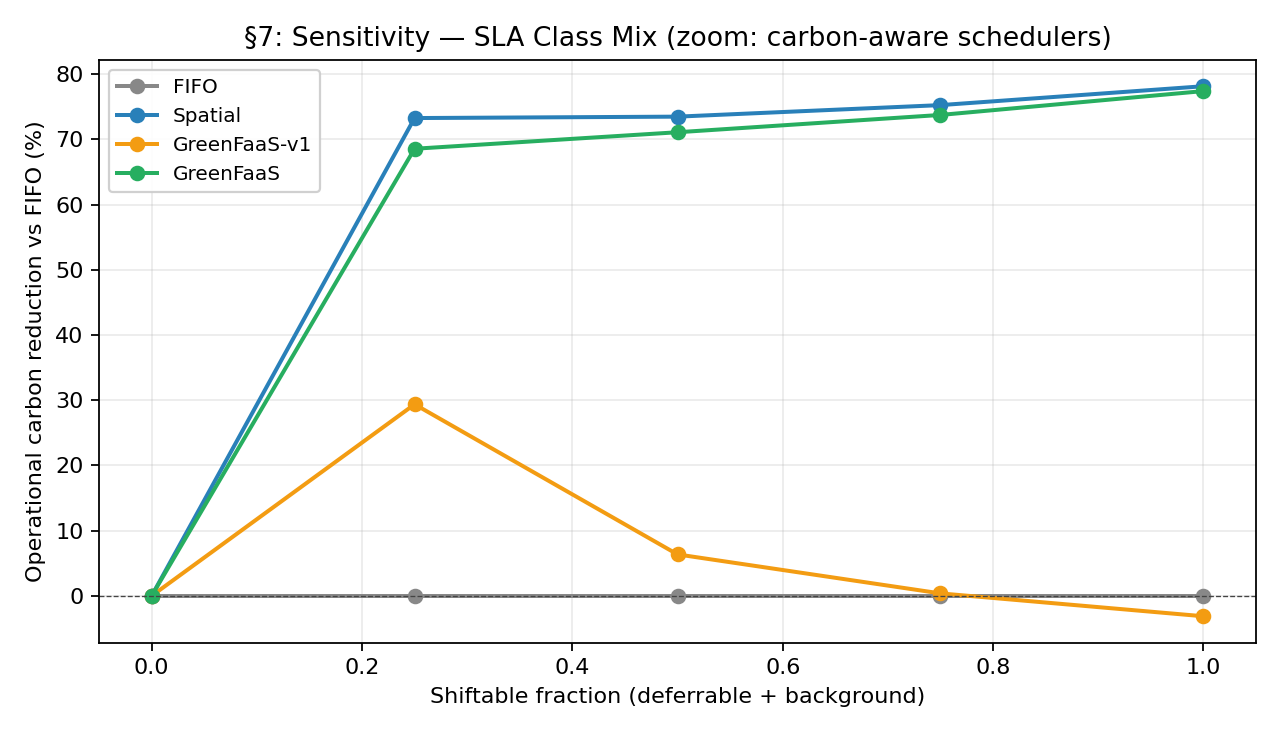
\includegraphics[width=\columnwidth]{figures/sensitivity_sla_mix_zoom.png}
\caption{Carbon reduction vs FIFO as the shiftable workload fraction
varies. \GreenFaaS{} climbs monotonically; GreenFaaS-v1 \emph{degrades}
as more shifting becomes available, the failure mode the
\S\ref{sec:tradeoff:idle} idle-energy correction was designed to
prevent.}
\label{fig:sla_mix}
\end{figure}

Three findings stand out. \emph{First}, all carbon-aware schedulers
correctly identify the 0\% shiftable case as offering no opportunity
and produce results identical to FIFO. \emph{Second}, Spatial and
\GreenFaaS{} both improve monotonically as the shiftable fraction
grows. \emph{Third}, \emph{GreenFaaS-v1 degrades
as more shifting becomes available}, dropping from $+29\%$ at 25\%
shiftable to $-3\%$ at 100\% shiftable. The v1 collapse is precisely
the failure mode the idle-energy correction was designed to prevent:
without charging the per-deferral idle cost, the scheduler aggressively
defers every eligible invocation, inflating warm-pool dwell times and
accumulating idle energy faster than it saves execution energy.

\subsection{Fine-Grained Do-No-Harm}
\label{sec:evaluation:fine-donoharm}

The do-no-harm property reported in
\S\ref{sec:evaluation:topology} and
\S\ref{sec:evaluation:realtopology} (\GreenFaaS{} = FIFO byte-for-byte
in single-region or zero-shiftable settings) admits a fair concern:
when the workload offers \emph{no} shifting opportunity, every
reasonable scheduler is trivially identical to FIFO. A more
substantive test is whether \GreenFaaS{} degrades \emph{gracefully}
across the regime of very small but nonzero shifting opportunity ---
where the scheduler actually has decisions to make but the carbon
upside is marginal, and a naively eager scheduler could pay
non-trivial idle-energy cost for negligible savings.

\begin{table}[h]
\centering\small
\caption{Fine-grained shiftable-fraction sweep. Real LWA carbon,
5 regions, 6h, $\sim$43k invocations. ``Gap'' is carbon reduction vs
FIFO (positive = better than FIFO).}
\label{tab:fine-donoharm}
\begin{tabular}{rrrrr}
\toprule
Shiftable frac. & FIFO (g) & GreenFaaS gap & v1 gap & Spatial gap \\
\midrule
0.00          & 6.20 & +0.00\%  & +0.00\%  & +0.00\%  \\
0.01          & 6.20 & +0.00\%  & +0.00\%  & +0.00\%  \\
0.02          & 6.20 & +0.00\%  & +0.00\%  & +0.00\%  \\
0.05          & 6.20 & +3.64\%  & +4.14\%  & +4.14\%  \\
0.10          & 6.20 & +3.64\%  & +4.14\%  & +4.14\%  \\
0.25          & 6.20 & +21.3\%  & +22.0\%  & +22.0\%  \\
\bottomrule
\end{tabular}
\end{table}

The findings refine the do-no-harm claim into something more
substantive. At very low shiftable fractions (0, 1\%, 2\% of the
workload), \GreenFaaS{}, GreenFaaS-v1, and Spatial all match FIFO
\emph{byte-for-byte}. This is not the trivial property
``no-shifting-implies-FIFO'' but the stronger property that
\GreenFaaS{} correctly identifies negligible-opportunity regimes and
declines to act. As the shiftable fraction grows past a small
threshold (around 5\% here), the carbon-aware schedulers begin
diverging from FIFO smoothly, with \GreenFaaS{} producing slightly
smaller savings than Spatial or v1 in this region --- the
\S\ref{sec:tradeoff:idle} correction is conservative when in doubt,
which is the desired behaviour for a deployment-ready scheduler.

The regime where \GreenFaaS{}'s conservatism becomes an advantage
appears at higher shiftable fractions where carbon variability is
high and idle-energy cost is non-trivial; the
\S\ref{sec:evaluation:variability} variability sweep (and the v1
collapse documented there) is the empirical evidence for this.

The interpretation: do-no-harm is not just ``correctly idle
when there are no decisions to make,'' but ``correctly idle across a
neighbourhood of low-opportunity workloads,'' which is the practical
shape of the property that matters for deployment.


\subsection{Sensitivity to Forecast Accuracy}
\label{sec:evaluation:forecast}

Several carbon-aware schedulers assume access to multi-hour
forecasts. We vary \GreenFaaS's forecast horizon across
\textsf{perfect}, \textsf{24h}, \textsf{1h}, \textsf{none}.

\GreenFaaS's carbon reduction is \emph{invariant} to forecast accuracy
across the four levels tested (69.5\% in all cases). The reason is
structural: the region-gating logic uses \emph{instantaneous} carbon
intensities (not forecasts), and the per-slot scoring is bounded by
the \Deferrable{} class's 60-second deferral horizon, which is
shorter than the carbon trace's 300-second resolution. Forecasts only
matter to \GreenFaaS{} for \Background{} invocations with multi-hour
deadlines, which are a minority of the canonical workload.

\paragraph{Scope of this invariance.} We note a
caveat: in our setup the carbon-trace step size (300\,s) exceeds the
\Deferrable{} class's deferral horizon (60\,s), which means that for
the dominant \Deferrable{} class, $N_{\text{slots}} = 1$ and the
forecast is never actually consulted. The invariance result is
therefore partially a consequence of forecast-temporal-resolution
exceeding the deferral horizon, not solely a structural property of
the scheduler. With higher-resolution carbon data (1-minute
ElectricityMaps feeds, for instance, where $N_{\text{slots}} \approx
60$ becomes feasible), \GreenFaaS{} would consult the forecast for
\Deferrable{} invocations, and forecast sensitivity could appear.
\Background{} invocations \emph{do} exercise the multi-hour forecast
horizon and produce identical results across forecast accuracies,
which is the load-bearing portion of the invariance claim. The
precise statement is that \GreenFaaS{} is forecast-invariant
\emph{(a)} for the \Background{} class structurally, and
\emph{(b)} for the \Deferrable{} class under typical
carbon-trace resolutions; under higher-resolution forecast data the
\Deferrable{} class would consult the forecast and its sensitivity
remains to be characterized.

This forecast-robustness is a feature of the design even with the
caveat above. It substantially reduces the deployment complexity of
\GreenFaaS: a production rollout does not need to integrate with a
carbon-forecasting service, and degraded forecast quality during
incidents does not threaten behaviour. GreenFaaS-v1, by contrast,
shows substantial forecast sensitivity, ranging from 25.1\% at
\textsf{perfect} to 74.2\% at \textsf{none} --- another symptom of
the un-charged temporal deferral that the idle-energy correction
addresses.

\subsection{Sensitivity to Carbon-Intensity Variability}
\label{sec:evaluation:variability}

We vary the diurnal amplitude of every region's carbon trace from 0.0
(flat) to 0.75 (large swing), holding regional means and topology
fixed. The corrected \GreenFaaS{} sits in a narrow 69.8--71.7\% band
across the entire range, and Spatial in 74.1--74.7\%. \emph{Neither
scheduler is sensitive to diurnal amplitude} on this 5-region
topology, because the inter-region carbon ratio (FR 60 vs PL 700,
ratio $\sim 11.7\times$) dwarfs even a 75\% intra-region swing.

\begin{figure}[t]
\centering
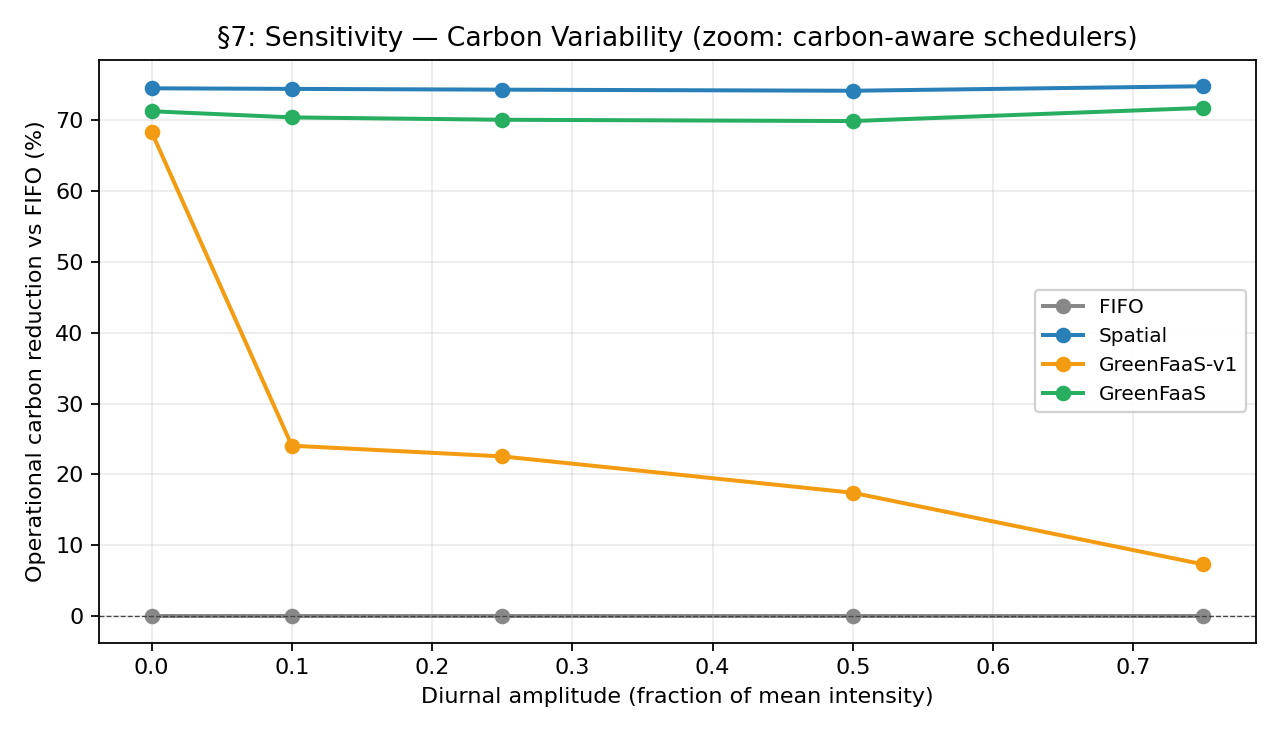
\includegraphics[width=\columnwidth]{figures/sensitivity_variability_zoom.png}
\caption{Carbon reduction as diurnal amplitude varies. The corrected
\GreenFaaS{} is stable. GreenFaaS-v1 \emph{degrades} with increasing
variability --- higher amplitude offers more deferral opportunities
that v1 incorrectly takes.}
\label{fig:variability}
\end{figure}

The v1 ablation (Figure~\ref{fig:variability}) shows a striking
\emph{negative} sensitivity: v1 falls from 68\% reduction at amplitude
0 to just 7\% at amplitude 0.75. Higher amplitude offers more
deferral opportunities that v1 incorrectly takes; the corrected
\GreenFaaS{} forgoes unprofitable deferrals and remains stable. This
is the second strong empirical validation of
\S\ref{sec:tradeoff:idle}.

\subsection{Sensitivity to Workload Intensity}
\label{sec:evaluation:intensity}

The fifth axis varies peak Poisson arrival rate from 0.5/s to 4.0/s
(an $8\times$ span). \GreenFaaS{} achieves 69.3--73.0\% reduction
across the range; Spatial achieves 70.9--84.4\%. The gap
\emph{narrows} with increasing intensity, from 11.4 percentage points
at 0.5/s to 1.6 at 4.0/s. Two mechanisms drive this convergence: at
higher rates Lemma~\ref{lemma:tradeoff}'s $\lambda^*$ is more readily
exceeded for more function-region pairs, so the region gate admits
more candidates; and the EWMA estimator's variance is lower at high
rates.

\subsection{Summary of Sensitivity Findings}
\label{sec:evaluation:summary}

Five axes yield five consistent findings.
\textbf{(1)} Wait-Awhile catastrophically fails on FaaS across every
setting, validating the paper's central claim that batch-oriented
schedulers do not transfer.
\textbf{(2)} Pure spatial routing captures most of the achievable
savings when a low-carbon refuge exists; \GreenFaaS{} matches Spatial
to within 1pp in these regimes.
\textbf{(3)} \GreenFaaS{} matches Spatial to within $1.3$pp across
all topologies including coal-belt, on \emph{both} synthetic and real
ENTSO-E 2020 carbon; instrumentation shows it performs no temporal
deferral on the coal-belt experiment, so its savings there are
spatial, not temporal
(\S\ref{sec:evaluation:topology}--\ref{sec:evaluation:realtopology}).
\textbf{(4)} \GreenFaaS{} preserves do-no-harm in single-region
topologies, low-variability traces, and at zero shiftable workload
fraction --- matching FIFO byte-for-byte when no axis offers real
savings.
\textbf{(5)} \GreenFaaS{} is robust to forecast quality and workload
intensity, with carbon reduction varying by less than 4 percentage
points across the tested ranges.

The GreenFaaS-v1 ablation makes the case for the
\S\ref{sec:tradeoff:idle} idle-energy correction crisp: without it,
the scheduler exhibits Wait-Awhile-like failure modes in milder form
(degradation under high shiftable fraction, under high carbon
variability, and in single-region topologies). With it, \GreenFaaS{}
is robust across every tested axis.
